\documentclass{article}

\usepackage{mathtools,amsfonts}
\usepackage{amssymb}
\usepackage{enumerate}
\usepackage{fancyvrb}
\usepackage{graphicx}
% \usepackage{fullpage}
\graphicspath{ {./} }

\begin{document}

\begin{center}
  \textbf{\Large Junior Test 2 Solutions}
  % LEVEL is Advanced, Intermediate or Beginner
  % NUMBER is the test number: 1, 2, etc.
  \\ \vspace{1em}
  \textbf{\large Stellenbosch Camp 2019}
\end{center}


\begin{enumerate}[1.]

\item %Source of problem
\textit
{
    Tile an $8 \times 8$ chessboard with T-shaped tetrominoes.
}

\textit{Solution}: 
\begin{center}
    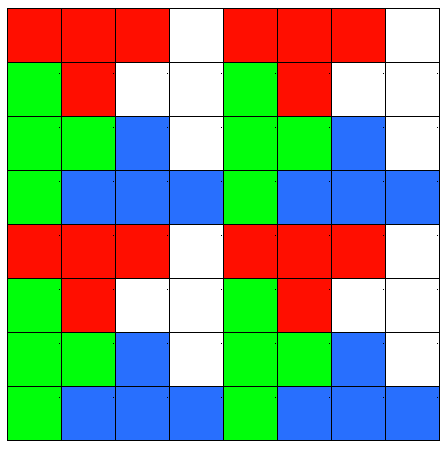
\includegraphics[scale=0.5]{tiling.png}
\end{center}

\item %Source
\textit{Prove that for all $a, b > 0$,
\[ \frac{a}{b} + \frac{b}{a} \geq 2. \]
}

\textit{Solution}:
$a, b > 0$, so $ab > 0$.
\begin{align*}
  &&\frac{a}{b} + \frac{b}{a} &\geq 2 \\
  &\iff& a^2 + b^2 &\geq 2ab \\
  &\iff& a^2 - 2ab + b^2 &\geq 0 \\
  &\iff& (a - b)^2 &\geq 0 & 
\end{align*}

The square of a real number is always non-negative, so it is true.

\item % Source
\textit{In $\triangle ABC$ let $\angle ACB = 90^\circ$, $AC = 1$ and $AB = 2$.
Let $M$ be the midpoint of $AB$ and $D$ the intersection of the angle bisector of $\angle CAB$ and $BC$.
Prove that $AB \perp CM$.
}

\textit{Solution}:
Notice that $\triangle ABC$ is a special triangle with angles $90^\circ$, $60^\circ$, and $30^\circ$.

$\therefore DM \perp AB$ and $DM = CD = \frac{\sqrt{3}}{3} $.

$\therefore ACDM$ is a kite.

$\therefore AD \perp MC$.


\item % Source
\textit{Find the first number which appears in all 3 the following arithmetic progressions:
\begin{center}
	$21, 34, 57, 70,...$\\
	$33, 37, 41, 45,...$\\
	$42, 75, 108, 141,...$
\end{center}}

\textit{Solution}:
Let $M$ be the smallest such number

\begin{align*}
\therefore M &\equiv _{13} 8 \\
M &\equiv _{4} 1 \\
M &\equiv _{33} 9
\end{align*}

$\therefore M = m_1(4 \cdot 33)(8) + m_2(13 \cdot 33)(1) + m_3(13 \cdot 4)(9) + n(4 \cdot 13 \cdot 33)$.
\begin{align*}
  &\therefore& m_1(4 \cdot 33) &\equiv _{13} 1 &\implies& m_1 = 7 \\
  &\therefore& m_2(13 \cdot 33) &\equiv _{4} 1 &\implies& m_2 = 1 \\
  &\therefore& m_3(4 \cdot 13) &\equiv _{33} 1 &\implies& m_3 = 7 
\end{align*}

$\therefore M = (7)(4 \cdot 33)(8) + (1)(13 \cdot 33)(1) + (7)(13 \cdot 4)(9) + n(4 \cdot 33 \cdot 13)$.

$\therefore M = 801$.


\item % Source
\textit{There are 7 people A, B, C, D, E, F, and G sitting in a row. B wants to sit next to C and E wants to sit next to F. How many different seating arrangements are there?
}

\textit{Solution}:
We can box $B$ and $C$ together considering them as a single entity which can appear in $2!$ ways ($BC$ or $CB$). Similarly, we can group $E$ and $F$ into a single entity. This means that the total number of combinations if $5! \cdot 2! \cdot 2! = 480$.


\item % Source
\textit{Given $\triangle ABC$, with $AB < AC$, let D be the point where the angle bisector of $angle BAC$ intersects the circumcircle of $\triangle ABC$.
Let $P$ and $Q$ be the altitudes dropped onto the extensions of $AB$ and $AC$.
Prove that $PB = QC$.
}

\textit{Solution}:
Construct lines $DB$ and $DC$, note that $DB = DC$ as they subtend the same angle.

Additionally, $PD = DQ$ since $\triangle APD \equiv \triangle AQD$.

$\therefore \triangle BPD \equiv \triangle CQD$ (RHS).

$\therefore BP = QC$.


\item % Source
\textit{What are the last two digits of $7^{7^{7^{7}}}$?}

\textit{Solution}:
Note $7^4 \equiv _{100} 1$.

$\therefore 7^{7^{7^7}} \equiv _{100} (7^4)^k \cdot 7^r$

where $r \equiv _4 7{7^7}$.

$\therefore r \equiv _4 (-1)^{7^7} \equiv _4 -1 \equiv _4 3$

\begin{align*}
\therefore 7^{7^{7^7}} &\equiv _{100} (7^4)^k \cdot 7^3 \\
&\equiv _{100} (1)^k \cdot 7^3 \\
&\equiv _{100} 43
\end{align*}


\item % Source
\textit{Prove that for all $a, b, c, d > 0$,
\[ (a + b + c + d)^{4} \geq abcd \times 4^{4}. \]
}

\textit{Solution}:
Note that for $x$, $y > 0$ we have 
\begin{align*}
  && (x - y)^2 &\ge 0 \\
  &\implies& x^2 - 2xy + y^2 &\ge 0 \\
  &\implies& x^2 + y^2 &\ge 2xy \\
  &\implies& \frac{x^2 + y^2}{2} &\ge xy
\end{align*}

Now, we let $x^2 = \frac{a + b}{2}$ and $y^2 = \frac{c + d}{2}$.

\begin{align*}
  \frac{ \frac{a + b}{2} + \frac{c + d}{2} }{2} &\ge \sqrt{ ( \frac{a + b}{2} )( \frac{c + d}{2} ) } \\
  \frac{a + b + c + d}{4} &\ge \sqrt{ ( \frac{a + b}{2} )( \frac{c + d}{2} )} \\
  &\ge \sqrt{ \sqrt{ab} \sqrt{cd} } \\
  &\ge \sqrt[4]{abcd} \\
  \therefore (a + b + c + d) &\ge 4\sqrt[4]{abcd} \\ 
  \therefore (a + b + c + d)^4 &\ge abcd \times 4^4
\end{align*}

\item % Source
\textit{Given the smiley face colouring, can the board be made completely white through some order of inverting rows.
}

\textit{Solution}:
Let every white squre be denoted by a $1$, and every black square by a $-1$. Let $k$ be the product of all of the values in the grid. 
Note that an inversion of a row or column would never change the value of $k$, as you are multiplying each item in the row by $(-1)$ when you invert. Hence, $k$ gets multiplied by $(-1)^8 = 1$.

Note that in the original diagram, $k = -1$ and a completely white board will have $k = 1$. Since inversions do not change the value of $k$ for the board, it must be impossible.


\item % , 2018 December Monthly Assignment Q1
\textit{Let $n$ be a positive integer greater than 2. Let $r_1$ be the smallest odd divisor of $n$ greater than $1$ and let $r_2$ be the largest odd divisor of $n$. Find all $n$ such that
	\begin{center}
		$n=5r_{1}+3r_{2}$
\end{center}}

\textit{Solution}:
First notice that $r_{1}$ must be prime otherwise there is a smaller odd number that divides $n$. Let $2^k$ be the highest power of $2$ that divides $n$ and so we may write the given condition as 
$$2^kr_{1}p=5r_{1}+3r_{1}p$$
 for some odd number $p$. 
 
 If $p=1$ then the equation becomes $2^kr_{1}=8r_1$ so $k=3$, therefore $n=8r_{1}$ satisfies this for any odd prime $r_1$. 
 
 If $p\ge 3  $, $r_2=pr_{1}$ and so we have 
 \begin{align*}
 &&2^kr_{1}p &=5r_{1}+3pr_{1} \\
 &\implies& 2^kp &=5+3p \\
 &\implies& p(2^{k}-3) &=5 &
 \end{align*}
 
 and since $p\ge 3$, $p$ must be $5$ and $k$ must be $2$. So $n=20r_1$ for some odd prime not greater than $3$ and so $n=60$ and $n=100$ are valid.  


\end{enumerate}

\end{document}
